\chapter{矩阵}

\index{矩阵}

\key{矩阵}是一个数学概念，
在编程中对应于二维数组。
例如，
\[
A = 
 \begin{bmatrix}
  6 & 13 & 7 & 4 \\
  7 & 0 & 8 & 2 \\
  9 & 5 & 4 & 18 \\
 \end{bmatrix}
\]
是一个大小为 $3 \times 4$ 的矩阵，即
它有3行4列。
记号 $[i,j]$ 表示矩阵中
第 $i$ 行第 $j$ 列的元素。
例如，在上面的矩阵中，
$A[2,3]=8$ 且 $A[3,1]=9$。

\index{向量}

矩阵的一个特例是\key{向量}，
即大小为 $n \times 1$ 的一维矩阵。
例如，
\[
V =
\begin{bmatrix}
4 \\
7 \\
5 \\
\end{bmatrix}
\]
是一个包含三个元素的向量。

\index{转置}

矩阵 $A$ 的\key{转置} $A^T$ 是将 $A$ 的行和列
互换后得到的，即 $A^T[i,j]=A[j,i]$：
\[
A^T = 
 \begin{bmatrix}
  6 & 7 & 9 \\
  13 & 0 & 5 \\
  7 & 8 & 4 \\
  4 & 2 & 18 \\
 \end{bmatrix}
\]

\index{方阵}

如果一个矩阵的行数和列数相同，
则它是一个\key{方阵}。
例如，以下矩阵是一个方阵：

\[
S = 
 \begin{bmatrix}
  3 & 12 & 4  \\
  5 & 9 & 15  \\
  0 & 2 & 4 \\
 \end{bmatrix}
\]

\section{运算}

矩阵 $A$ 和 $B$ 的和 $A+B$ 只有在
两个矩阵大小相同时才有定义。
结果矩阵中每个元素是 $A$ 和 $B$ 中
对应元素之和。

例如，
\[
 \begin{bmatrix}
  6 & 1 & 4 \\
  3 & 9 & 2 \\
 \end{bmatrix}
+
 \begin{bmatrix}
  4 & 9 & 3 \\
  8 & 1 & 3 \\
 \end{bmatrix}
=
 \begin{bmatrix}
  6+4 & 1+9 & 4+3 \\
  3+8 & 9+1 & 2+3 \\
 \end{bmatrix}
=
 \begin{bmatrix}
  10 & 10 & 7 \\
  11 & 10 & 5 \\
 \end{bmatrix}.
\]

将矩阵 $A$ 乘以一个值 $x$ 意味着
$A$ 的每个元素都乘以 $x$。
例如，
\[
 2 \cdot \begin{bmatrix}
  6 & 1 & 4 \\
  3 & 9 & 2 \\
 \end{bmatrix}
=
 \begin{bmatrix}
  2 \cdot 6 & 2\cdot1 & 2\cdot4 \\
  2\cdot3 & 2\cdot9 & 2\cdot2 \\
 \end{bmatrix}
=
 \begin{bmatrix}
  12 & 2 & 8 \\
  6 & 18 & 4 \\
 \end{bmatrix}.
\]

\subsubsection{矩阵乘法}

\index{矩阵乘法}

矩阵 $A$ 和 $B$ 的乘积 $AB$ 只有在
$A$ 的大小为 $a \times n$ 且
$B$ 的大小为 $n \times b$ 时才有定义，
即 $A$ 的宽度等于 $B$ 的高度。
结果是一个大小为 $a \times b$ 的矩阵，
其元素由以下公式计算：
\[
AB[i,j] = \sum_{k=1}^n A[i,k] \cdot B[k,j].
\]

其思想是 $AB$ 的每个元素
是 $A$ 和 $B$ 的元素的乘积之和，
如下图所示：

\begin{center}
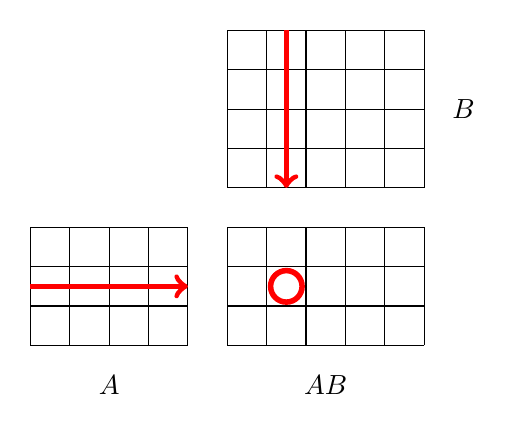
\begin{tikzpicture}[scale=0.5]
\draw (0,0) grid (4,3);
\draw (5,0) grid (10,3);
\draw (5,4) grid (10,8);

\node at (2,-1) {$A$};
\node at (7.5,-1) {$AB$};
\node at (11,6) {$B$};

\draw[thick,->,red,line width=2pt] (0,1.5) -- (4,1.5);
\draw[thick,->,red,line width=2pt] (6.5,8) -- (6.5,4);
\draw[thick,red,line width=2pt] (6.5,1.5) circle (0.4);
\end{tikzpicture}
\end{center}

例如，

\[
 \begin{bmatrix}
  1 & 4 \\
  3 & 9 \\
  8 & 6 \\
 \end{bmatrix}
\cdot
 \begin{bmatrix}
  1 & 6 \\
  2 & 9 \\
 \end{bmatrix}
=
 \begin{bmatrix}
  1 \cdot 1 + 4 \cdot 2 & 1 \cdot 6 + 4 \cdot 9 \\
  3 \cdot 1 + 9 \cdot 2 & 3 \cdot 6 + 9 \cdot 9 \\
  8 \cdot 1 + 6 \cdot 2 & 8 \cdot 6 + 6 \cdot 9 \\
 \end{bmatrix}
=
 \begin{bmatrix}
  9 & 42 \\
  21 & 99 \\
  20 & 102 \\
 \end{bmatrix}.
\]

矩阵乘法满足结合律，
即 $A(BC)=(AB)C$ 成立，
但不满足交换律，
即 $AB = BA$ 通常不成立。

\index{单位矩阵}

\key{单位矩阵}是一个方阵，
其主对角线上的每个元素为1，
其余所有元素为0。
例如，以下矩阵
是 $3 \times 3$ 单位矩阵：
\[
 I = \begin{bmatrix}
  1 & 0 & 0 \\
  0 & 1 & 0 \\
  0 & 0 & 1 \\
 \end{bmatrix}
\]

\begin{samepage}
将矩阵乘以单位矩阵不会改变它。例如，
\[
 \begin{bmatrix}
  1 & 0 & 0 \\
  0 & 1 & 0 \\
  0 & 0 & 1 \\
 \end{bmatrix}
\cdot
 \begin{bmatrix}
  1 & 4 \\
  3 & 9 \\
  8 & 6 \\
 \end{bmatrix}
=
 \begin{bmatrix}
  1 & 4 \\
  3 & 9 \\
  8 & 6 \\
 \end{bmatrix} \hspace{10pt} \textrm{和} \hspace{10pt}
 \begin{bmatrix}
  1 & 4 \\
  3 & 9 \\
  8 & 6 \\
 \end{bmatrix}
\cdot
 \begin{bmatrix}
  1 & 0 \\
  0 & 1 \\
 \end{bmatrix}
=
 \begin{bmatrix}
  1 & 4 \\
  3 & 9 \\
  8 & 6 \\
 \end{bmatrix}.
\]
\end{samepage}

使用直接算法，
我们可以计算两个
$n \times n$ 矩阵的乘积，
时间复杂度为 $O(n^3)$。
也有更高效的矩阵乘法算法\footnote{第一个这样的
算法是 Strassen 算法，
于1969年发表 \cite{str69}，
时间复杂度为 $O(n^{2.80735})$；
目前已知的最佳算法 \cite{gal14}
的时间复杂度为 $O(n^{2.37286})$。},
但它们主要具有理论意义，
在竞赛编程中不需要使用这样的算法。


\subsubsection{矩阵幂}

\index{矩阵幂}

矩阵 $A$ 的幂 $A^k$ 在
$A$ 为方阵时有定义。
其定义基于矩阵乘法：
\[ A^k = \underbrace{A \cdot A \cdot A \cdots A}_{\textrm{$k$ 次}} \]
例如，

\[
 \begin{bmatrix}
  2 & 5 \\
  1 & 4 \\
 \end{bmatrix}^3 =
 \begin{bmatrix}
  2 & 5 \\
  1 & 4 \\
 \end{bmatrix} \cdot
 \begin{bmatrix}
  2 & 5 \\
  1 & 4 \\
 \end{bmatrix} \cdot
 \begin{bmatrix}
  2 & 5 \\
  1 & 4 \\
 \end{bmatrix} =
 \begin{bmatrix}
  48 & 165 \\
  33 & 114 \\
 \end{bmatrix}.
\]
此外，$A^0$ 是单位矩阵。例如，
\[
 \begin{bmatrix}
  2 & 5 \\
  1 & 4 \\
 \end{bmatrix}^0 =
 \begin{bmatrix}
  1 & 0 \\
  0 & 1 \\
 \end{bmatrix}.
\]

矩阵 $A^k$ 可以使用第21.2章中的算法
在 $O(n^3 \log k)$ 时间内高效计算。例如，
\[
 \begin{bmatrix}
  2 & 5 \\
  1 & 4 \\
 \end{bmatrix}^8 =
 \begin{bmatrix}
  2 & 5 \\
  1 & 4 \\
 \end{bmatrix}^4 \cdot
 \begin{bmatrix}
  2 & 5 \\
  1 & 4 \\
 \end{bmatrix}^4.
\]

\subsubsection{行列式}

\index{行列式}

矩阵 $A$ 的\key{行列式} $\det(A)$ 只有在
$A$ 是方阵时才有定义。
如果 $A$ 的大小为 $1 \times 1$，
则 $\det(A)=A[1,1]$。
更大矩阵的行列式使用以下公式递归计算 \index{余子式}
\[\det(A)=\sum_{j=1}^n A[1,j] C[1,j],\]
其中 $C[i,j]$ 是 $A$ 在 $[i,j]$ 处的\key{余子式}。
余子式由以下公式计算：
\[C[i,j] = (-1)^{i+j} \det(M[i,j]),\]
其中 $M[i,j]$ 是从 $A$ 中去掉
第 $i$ 行和第 $j$ 列后得到的矩阵。
由于余子式中的系数 $(-1)^{i+j}$，
行列式的值交替为正和负。
例如，
\[
\det(
 \begin{bmatrix}
  3 & 4 \\
  1 & 6 \\
 \end{bmatrix}
) = 3 \cdot 6 - 4 \cdot 1 = 14
\]
和
\[
\det(
 \begin{bmatrix}
  2 & 4 & 3 \\
  5 & 1 & 6 \\
  7 & 2 & 4 \\
 \end{bmatrix}
) =
2 \cdot
\det(
 \begin{bmatrix}
  1 & 6 \\
  2 & 4 \\
 \end{bmatrix}
)
-4 \cdot
\det(
 \begin{bmatrix}
  5 & 6 \\
  7 & 4 \\
 \end{bmatrix}
)
+3 \cdot
\det(
 \begin{bmatrix}
  5 & 1 \\
  7 & 2 \\
 \end{bmatrix}
) = 81.
\]

\index{逆矩阵}

$A$ 的行列式告诉我们
是否存在\key{逆矩阵}
$A^{-1}$ 使得 $A \cdot A^{-1} = I$，
其中 $I$ 是单位矩阵。
结果表明，$A^{-1}$ 存在
当且仅当 $\det(A) \neq 0$，
且可以用以下公式计算：

\[A^{-1}[i,j] = \frac{C[j,i]}{det(A)}.\]

例如，

\[
\underbrace{
 \begin{bmatrix}
  2 & 4 & 3\\
  5 & 1 & 6\\
  7 & 2 & 4\\
 \end{bmatrix}
}_{A}
\cdot
\underbrace{
 \frac{1}{81}
 \begin{bmatrix}
   -8 & -10 & 21 \\
   22 & -13 & 3 \\
   3 & 24 & -18 \\
 \end{bmatrix}
}_{A^{-1}}
=
\underbrace{
 \begin{bmatrix}
  1 & 0 & 0 \\
  0 & 1 & 0 \\
  0 & 0 & 1 \\
 \end{bmatrix}
}_{I}.
\]

\section{线性递推}

\index{线性递推}

\key{线性递推}
是一个函数 $f(n)$，
其初始值为
$f(0),f(1),\ldots,f(k-1)$，
更大的值由以下公式递归计算：
\[f(n) = c_1 f(n-1) + c_2 f(n-2) + \ldots + c_k f (n-k),\]
其中 $c_1,c_2,\ldots,c_k$ 是常量系数。

可以使用动态规划在 $O(kn)$ 时间内
计算 $f(n)$ 的任意值，方法是依次计算
$f(0),f(1),\ldots,f(n)$ 的所有值。
然而，如果 $k$ 较小，可以使用矩阵运算
在 $O(k^3 \log n)$ 时间内更高效地
计算 $f(n)$。

\subsubsection{斐波那契数}

\index{斐波那契数}

线性递推的一个简单例子是
以下定义斐波那契数的函数：
\[
\begin{array}{lcl}
f(0) & = & 0 \\
f(1) & = & 1 \\
f(n) & = & f(n-1)+f(n-2) \\
\end{array}
\]
在这种情况下，$k=2$ 且 $c_1=c_2=1$。

\begin{samepage}
为了高效计算斐波那契数，
我们将斐波那契公式表示为
一个大小为 $2 \times 2$ 的方阵 $X$，
满足以下关系：
\[ X \cdot
 \begin{bmatrix}
  f(i) \\
  f(i+1) \\
 \end{bmatrix}
=
 \begin{bmatrix}
  f(i+1) \\
  f(i+2) \\
 \end{bmatrix}
 \]
因此，$f(i)$ 和 $f(i+1)$ 的值作为
$X$ 的''输入''，
而 $X$ 从中计算出 $f(i+1)$ 和 $f(i+2)$ 的值。
结果表明，这样的矩阵是

\[ X = 
 \begin{bmatrix}
  0 & 1 \\
  1 & 1 \\
 \end{bmatrix}.
\]
\end{samepage}
\noindent
例如，
\[
 \begin{bmatrix}
  0 & 1 \\
  1 & 1 \\
 \end{bmatrix}
\cdot
 \begin{bmatrix}
  f(5) \\
  f(6) \\
 \end{bmatrix}
=
 \begin{bmatrix}
  0 & 1 \\
  1 & 1 \\
 \end{bmatrix}
\cdot
 \begin{bmatrix}
  5 \\
  8 \\
 \end{bmatrix}
=
 \begin{bmatrix}
  8 \\
  13 \\
 \end{bmatrix}
=
 \begin{bmatrix}
  f(6) \\
  f(7) \\
 \end{bmatrix}.
\]
因此，我们可以使用以下公式计算 $f(n)$
\[
 \begin{bmatrix}
  f(n) \\
  f(n+1) \\
 \end{bmatrix}
=
X^n \cdot
 \begin{bmatrix}
  f(0) \\
  f(1) \\
 \end{bmatrix}
=
 \begin{bmatrix}
  0 & 1 \\
  1 & 1 \\
 \end{bmatrix}^n
\cdot
 \begin{bmatrix}
  0 \\
  1 \\
 \end{bmatrix}.
\]
$X^n$ 的值可以在
$O(\log n)$ 时间内计算，
因此 $f(n)$ 的值也可以在
$O(\log n)$ 时间内计算。

\subsubsection{一般情况}

现在考虑一般情况，
其中 $f(n)$ 是任意线性递推。
同样，我们的目标是构造一个矩阵 $X$，
使得

\[ X \cdot
 \begin{bmatrix}
  f(i) \\
  f(i+1) \\
  \vdots \\
  f(i+k-1) \\
 \end{bmatrix}
=
 \begin{bmatrix}
  f(i+1) \\
  f(i+2) \\
  \vdots \\
  f(i+k) \\
 \end{bmatrix}.
\]
这样的矩阵是
\[
X =
 \begin{bmatrix}
  0 & 1 & 0 & 0 & \cdots & 0 \\
  0 & 0 & 1 & 0 & \cdots & 0 \\
  0 & 0 & 0 & 1 & \cdots & 0 \\
  \vdots & \vdots & \vdots & \vdots & \ddots & \vdots \\
  0 & 0 & 0 & 0 & \cdots & 1 \\
  c_k & c_{k-1} & c_{k-2} & c_{k-3} & \cdots & c_1 \\
 \end{bmatrix}.
\]
在前 $k-1$ 行中，每个元素为0，
除了一个元素为1。
这些行将 $f(i)$ 替换为 $f(i+1)$，
$f(i+1)$ 替换为 $f(i+2)$，以此类推。
最后一行包含递推的系数，
用于计算新值 $f(i+k)$。

\begin{samepage}
现在，可以使用以下公式
在 $O(k^3 \log n)$ 时间内计算 $f(n)$
\[
 \begin{bmatrix}
  f(n) \\
  f(n+1) \\
  \vdots \\
  f(n+k-1) \\
 \end{bmatrix}
=
X^n \cdot
 \begin{bmatrix}
  f(0) \\
  f(1) \\
  \vdots \\
  f(k-1) \\
 \end{bmatrix}.
\]
\end{samepage}

\section{图与矩阵}

\subsubsection{路径计数}

图的邻接矩阵的幂有一个有趣的性质。
当 $V$ 是一个无权图的邻接矩阵时，
矩阵 $V^n$ 包含图中节点之间
经过 $n$ 条边的路径数量。

例如，对于图
\begin{center}
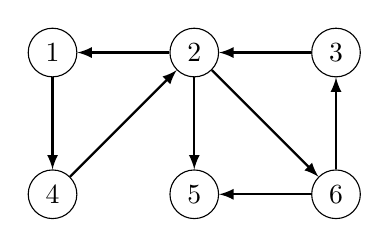
\begin{tikzpicture}[scale=0.9]
\node[draw, circle] (1) at (1,3) {$1$};
\node[draw, circle] (2) at (1,1) {$4$};
\node[draw, circle] (3) at (3,3) {$2$};
\node[draw, circle] (4) at (5,3) {$3$};
\node[draw, circle] (5) at (3,1) {$5$};
\node[draw, circle] (6) at (5,1) {$6$};

\path[draw,thick,->,>=latex] (1) -- (2);
\path[draw,thick,->,>=latex] (2) -- (3);
\path[draw,thick,->,>=latex] (3) -- (1);
\path[draw,thick,->,>=latex] (4) -- (3);
\path[draw,thick,->,>=latex] (3) -- (5);
\path[draw,thick,->,>=latex] (3) -- (6);
\path[draw,thick,->,>=latex] (6) -- (4);
\path[draw,thick,->,>=latex] (6) -- (5);
\end{tikzpicture}
\end{center}
邻接矩阵为
\[
V= \begin{bmatrix}
  0 & 0 & 0 & 1 & 0 & 0 \\
  1 & 0 & 0 & 0 & 1 & 1 \\
  0 & 1 & 0 & 0 & 0 & 0 \\
  0 & 1 & 0 & 0 & 0 & 0 \\
  0 & 0 & 0 & 0 & 0 & 0 \\
  0 & 0 & 1 & 0 & 1 & 0 \\
 \end{bmatrix}.
\]
现在，例如，矩阵
\[
V^4= \begin{bmatrix}
  0 & 0 & 1 & 1 & 1 & 0 \\
  2 & 0 & 0 & 0 & 2 & 2 \\
  0 & 2 & 0 & 0 & 0 & 0 \\
  0 & 2 & 0 & 0 & 0 & 0 \\
  0 & 0 & 0 & 0 & 0 & 0 \\
  0 & 0 & 1 & 1 & 1 & 0 \\
 \end{bmatrix}
\]
包含了节点之间
经过4条边的路径数量。
例如，$V^4[2,5]=2$，
因为从节点2到节点5有两条经过4条边的路径：
$2 \rightarrow 1 \rightarrow 4 \rightarrow 2 \rightarrow 5$
和
$2 \rightarrow 6 \rightarrow 3 \rightarrow 2 \rightarrow 5$。

\subsubsection{最短路径}

在加权图中使用类似的思想，
我们可以计算每对节点之间
恰好包含 $n$ 条边的路径的最小长度。
为此，我们需要以新的方式定义矩阵乘法，
使得我们不是计算路径数量，
而是最小化路径长度。

\begin{samepage}
作为一个例子，考虑以下图：
\begin{center}
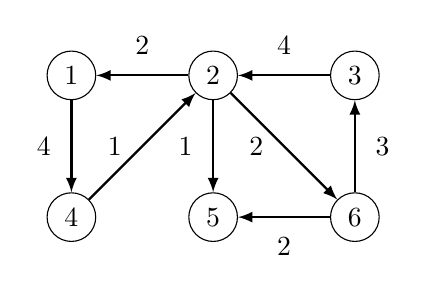
\begin{tikzpicture}[scale=0.9]
\node[draw, circle] (1) at (1,3) {$1$};
\node[draw, circle] (2) at (1,1) {$4$};
\node[draw, circle] (3) at (3,3) {$2$};
\node[draw, circle] (4) at (5,3) {$3$};
\node[draw, circle] (5) at (3,1) {$5$};
\node[draw, circle] (6) at (5,1) {$6$};

\path[draw,thick,->,>=latex] (1) -- node[font=\small,label=left:4] {} (2);
\path[draw,thick,->,>=latex] (2) -- node[font=\small,label=left:1] {} (3);
\path[draw,thick,->,>=latex] (3) -- node[font=\small,label=north:2] {} (1);
\path[draw,thick,->,>=latex] (4) -- node[font=\small,label=north:4] {} (3);
\path[draw,thick,->,>=latex] (3) -- node[font=\small,label=left:1] {} (5);
\path[draw,thick,->,>=latex] (3) -- node[font=\small,label=left:2] {} (6);
\path[draw,thick,->,>=latex] (6) -- node[font=\small,label=right:3] {} (4);
\path[draw,thick,->,>=latex] (6) -- node[font=\small,label=below:2] {} (5);
\end{tikzpicture}
\end{center}
\end{samepage}

我们构造一个邻接矩阵，其中
$\infty$ 表示边不存在，
其他值对应边权重。
该矩阵为
\[
V= \begin{bmatrix}
  \infty & \infty & \infty & 4 & \infty & \infty \\
  2 & \infty & \infty & \infty & 1 & 2 \\
  \infty & 4 & \infty & \infty & \infty & \infty \\
  \infty & 1 & \infty & \infty & \infty & \infty \\
  \infty & \infty & \infty & \infty & \infty & \infty \\
  \infty & \infty & 3 & \infty & 2 & \infty \\
 \end{bmatrix}.
\]

现在我们不使用公式
\[
AB[i,j] = \sum_{k=1}^n A[i,k] \cdot B[k,j]
\]
而是使用公式
\[
AB[i,j] = \min_{k=1}^n A[i,k] + B[k,j]
\]
进行矩阵乘法，即我们计算
最小值而非求和，
元素之和而非乘积。
经过这个修改后，
矩阵的幂对应于图中的最短路径。

例如，由于
\[
V^4= \begin{bmatrix}
  \infty & \infty & 10 & 11 & 9 & \infty \\
  9 & \infty & \infty & \infty & 8 & 9 \\
  \infty & 11 & \infty & \infty & \infty & \infty \\
  \infty & 8 & \infty & \infty & \infty & \infty \\
  \infty & \infty & \infty & \infty & \infty & \infty \\
  \infty & \infty & 12 & 13 & 11 & \infty \\
 \end{bmatrix},
\]
我们可以得出结论，从节点2到节点5
经过4条边的路径的最小长度为8。
这样的路径是
$2 \rightarrow 1 \rightarrow 4 \rightarrow 2 \rightarrow 5$。

\subsubsection{基尔霍夫定理}

\index{基尔霍夫定理}
\index{生成树}

\key{基尔霍夫定理}
%\footnote{G. R. Kirchhoff (1824--1887) was a German physicist.}
提供了一种方法，
可以通过一个特殊矩阵的行列式
来计算图的生成树数量。
例如，图
\begin{center}
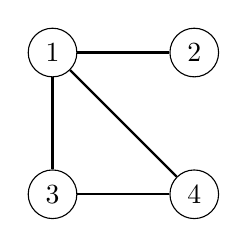
\begin{tikzpicture}[scale=0.9]
\node[draw, circle] (1) at (1,3) {$1$};
\node[draw, circle] (2) at (3,3) {$2$};
\node[draw, circle] (3) at (1,1) {$3$};
\node[draw, circle] (4) at (3,1) {$4$};

\path[draw,thick,-] (1) -- (2);
\path[draw,thick,-] (1) -- (3);
\path[draw,thick,-] (3) -- (4);
\path[draw,thick,-] (1) -- (4);
\end{tikzpicture}
\end{center}
有三棵生成树：
\begin{center}
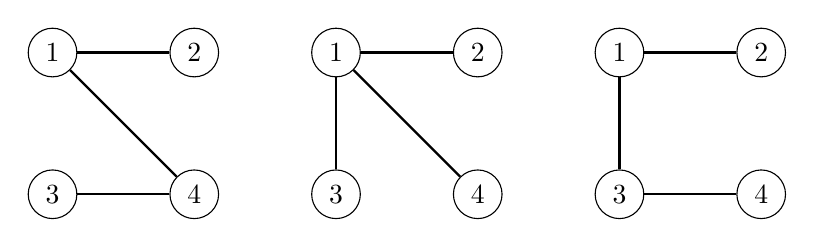
\begin{tikzpicture}[scale=0.9]
\node[draw, circle] (1a) at (1,3) {$1$};
\node[draw, circle] (2a) at (3,3) {$2$};
\node[draw, circle] (3a) at (1,1) {$3$};
\node[draw, circle] (4a) at (3,1) {$4$};

\path[draw,thick,-] (1a) -- (2a);
%\path[draw,thick,-] (1a) -- (3a);
\path[draw,thick,-] (3a) -- (4a);
\path[draw,thick,-] (1a) -- (4a);

\node[draw, circle] (1b) at (1+4,3) {$1$};
\node[draw, circle] (2b) at (3+4,3) {$2$};
\node[draw, circle] (3b) at (1+4,1) {$3$};
\node[draw, circle] (4b) at (3+4,1) {$4$};

\path[draw,thick,-] (1b) -- (2b);
\path[draw,thick,-] (1b) -- (3b);
%\path[draw,thick,-] (3b) -- (4b);
\path[draw,thick,-] (1b) -- (4b);

\node[draw, circle] (1c) at (1+8,3) {$1$};
\node[draw, circle] (2c) at (3+8,3) {$2$};
\node[draw, circle] (3c) at (1+8,1) {$3$};
\node[draw, circle] (4c) at (3+8,1) {$4$};

\path[draw,thick,-] (1c) -- (2c);
\path[draw,thick,-] (1c) -- (3c);
\path[draw,thick,-] (3c) -- (4c);
%\path[draw,thick,-] (1c) -- (4c);
\end{tikzpicture}
\end{center}
\index{拉普拉斯矩阵}
为了计算生成树的数量，
我们构造一个\key{拉普拉斯矩阵} $L$，
其中 $L[i,i]$ 是节点 $i$ 的度数，
如果节点 $i$ 和 $j$ 之间有边，
则 $L[i,j]=-1$，否则 $L[i,j]=0$。
上述图的拉普拉斯矩阵如下：
\[
L= \begin{bmatrix}
  3 & -1 & -1 & -1 \\
  -1 & 1 & 0 & 0 \\
  -1 & 0 & 2 & -1 \\
  -1 & 0 & -1 & 2 \\
 \end{bmatrix}
\]

可以证明，
生成树的数量等于从 $L$ 中
去掉任意一行和任意一列后得到的矩阵的行列式。
例如，如果我们去掉第一行和第一列，结果是

\[ \det(
\begin{bmatrix}
  1 & 0 & 0 \\
  0 & 2 & -1 \\
  0 & -1 & 2 \\
 \end{bmatrix}
) =3.\]
行列式总是相同的，
无论我们从 $L$ 中去掉哪一行和哪一列。

注意，第22.5章中的凯莱公式
是基尔霍夫定理的一个特例，
因为在 $n$ 个节点的完全图中

\[ \det(
\begin{bmatrix}
  n-1 & -1 & \cdots & -1 \\
  -1 & n-1 & \cdots & -1 \\
  \vdots & \vdots & \ddots & \vdots \\
  -1 & -1 & \cdots & n-1 \\
 \end{bmatrix}
) =n^{n-2}.\]



